\documentclass[oneside]{book}

\usepackage[utf8]{inputenc}
\usepackage{graphicx}
\usepackage{subfig}
\usepackage{color}
\usepackage{soul}
\usepackage{xspace}
\usepackage{multirow}
\usepackage{alltt}
\usepackage{url}
\usepackage{amssymb}
\usepackage{amsthm}
\usepackage[english]{babel}
\usepackage[T1]{fontenc}%da non usare nella versione camera-ready
\usepackage{multirow}
\usepackage{amsmath}% ci serve per la H piccola in datalog^E,H
\usepackage{arydshln}
\usepackage{booktabs}
\DeclareMathAlphabet{\mathbb}{U}{fplmbb}{bb}{it}

\usepackage[normalem]{ulem}
\usepackage{amsmath}
\newcommand{\stkout}[1]{\ifmmode\text{\sout{\ensuremath{#1}}}\else\sout{#1}\fi}

\usepackage[]{hyperref}

\usepackage{parskip}
\usepackage{listings}
\usepackage{enumitem}


\usepackage[colorinlistoftodos,textwidth=160pt]{todonotes}
\presetkeys{todonotes}{color=blue!20, bordercolor=blue!80}{}
\newcommand{\ste}[1]{\todo[color=green!40, bordercolor=green!80, author=Stefano]{#1}{}}

%\makeatletter\@addtoreset{chapter}{part}\makeatother%

\usepackage[top=1in, bottom=1.25in, left=1.25in, right=1.25in]{geometry}

% \makeatletter
% \@addtoreset{chapter}{part}
% \makeatother

\begin{document}

\title{\bf Enhancing the DLV system for\\large-scale ontology reasoning \\ \ \\
\Large \em Preliminary Report
\\ \ \\ }
\author{xxxx}

%\date{December 2004}
\maketitle

\pagenumbering{Roman}

\chapter*{Summary}
%\addcontentsline{toc}{chapter}{Abstract}
The summary goes here...


\tableofcontents
\listoffigures
\listoftables


\chapter*{Introduction}
\addcontentsline{toc}{chapter}{\numberline{}Introduction}
\markright{Introduction}
\pagenumbering{arabic}

%\renewcommand{\abstractname}{Executive Summary}
% \begin{abstract}
% \addcontentsline{toc}{chapter}{Abstract}
% The abstract goes here...
% ...
% \end{abstract}

%%%%%%%%%%%%%%%%%%%%%%%%%%%%%%%%%%%%%%%%%%%%%%%%%%%%%%%%%%%%%%%%%%%%%%%%%%%%%%%%%%%%%%%%%%%%%%%%%%%%%%%%%%%%%%%%%%%%%%%%
%%%%%%%%%%%%%%%%%%%%%%%%%%%%%%%%%%%%%%%%%%%%%%%%%%%%%%%%%%%%%%%%%%%%%%%%%%%%%%%%%%%%%%%%%%%%%%%%%%%%%%%%%%%%%%%%%%%%%%%%
%%%%%%%%%%%%%%%%%%%%%%%%%%%%%%%%%%%%%%%%%%%%%%%%%%%%%%%%%%%%%%%%%%%%%%%%%%%%%%%%%%%%%%%%%%%%%%%%%%%%%%%%%%%%%%%%%%%%%%%%



\part*{Work Package 1:\\Data Loading Procedure Extensions}
\addcontentsline{toc}{part}{WP1: Data Loading Procedure Extensions}

\chapter{Scenario and problem description}

DLV natively supports the ASP formalism that requires data to be represented as a set of relational facts. One of the goals of this project is to extend the system in order to deal with OWL TBoxes in RDF/XML format, RDF ABoxes in Turtle format and Conjunctive Queries in SPARQL. In particular, a ``rewriting-based'' approach for handling OWL ontologies and SPARQL queries will be designed and developed within WP2; whereas, an extension of the system for loading Turtle ABoxes has been developed within WP1. 
BLA BLA BLA…\ste{Fix introduction}

\section{Team}
WP1 has been fully developed by DLVSystem. In particular, what follows is the list of the involved researchers: Stefano Germano (PostDoc), Pierfrancesco Veltri (PostDoc), Jessica Zangari (PostDoc).



\section{The Turtle standard - Terse RDF Triple Language\texorpdfstring{\protect\footnote{From~\url{https://www.w3.org/TR/turtle}}}{}}

We refer to RDF 1.1 Turtle as reported in its latest published version, available at \url{http://www.w3.org/TR/2014/REC-turtle-20140225/}.

The Resource Description Framework (RDF) is a general-purpose language for representing information in the Web.
We use a textual syntax for RDF called Turtle that allows an RDF graph to be completely written in a compact and natural text form, with abbreviations for common usage patterns and datatypes.

A Turtle document allows writing down an RDF graph in a compact textual form. An RDF graph is made up of triples consisting of a subject, predicate and object.\\
Comments may be given after a '\#' that is not part of another lexical token and continue to the end of the line.

The simplest triple statement is a sequence of (subject, predicate, object) terms, separated by whitespace and terminated by '.' after each triple.

Often the same subject will be referenced by a number of predicates. The predicateObjectList production matches a series of predicates and objects, separated by ';', following a subject. This expresses a series of RDF Triples with that subject and each predicate and object allocated to one triple. Thus, the ';' symbol is used to repeat the subject of triples that vary only in predicate and object RDF terms.
As with predicates often objects are repeated with the same subject and predicate. The objectList production matches a series of objects separated by ',' following a predicate. This expresses a series of RDF Triples with the corresponding subject and predicate and each object allocated to one triple. Thus, the ',' symbol is used to repeat the subject and predicate of triples that only differ in the object RDF term.

IRIs may be written as relative or absolute IRIs or prefixed names. Relative and absolute IRIs are enclosed in '<' and '>'.\\
Relative IRIs are resolved relative to the current base IRI. A new base IRI can be defined using the '@base' or 'BASE' directive.\\
The token 'a' in the predicate position of a Turtle triple represents the IRI\\
\verb|http://www.w3.org/1999/02/22-rdf-syntax-ns#type|.\\
A prefixed name is a prefix label and a local part, separated by a colon ":". A prefixed name is turned into an IRI by concatenating the IRI associated with the prefix and the local part. The '@prefix' or 'PREFIX' directive associates a prefix label with an IRI. Subsequent '@prefix' or 'PREFIX' directives may re-map the same prefix label.

Literals are used to identify values such as strings, numbers, dates.\\
Quoted Literals have a lexical form followed by a language tag, a datatype IRI, or neither.

\section{State of the art of Turtle parsing in C++}

\subsection{RDF Turtle management tools in C++}
There are C++ tools which provide parsing, serialising and management of RDF triples in the Turtle format.

The advantages of using an existing (and widely-used) tool are the stability, the correctness and the performance. The main disadvantage is the difficulty in customizing and adapting it to our needs (for example in terms of memory and time performance).

The most well-known (and widely-used) is the \href{http://librdf.org/raptor}{Raptor RDF Syntax Library}.\\
However, the latest version of this library is from 2014.\\
Moreover, their ``Turtle Parser'' is outdated; \href{https://www.w3.org/TR/turtle}{the latest version of the standard is from 2014} but they support an older one, as reported in their documentation:
\begin{quote}
\textit{A parser for the \href{http://www.w3.org/TR/2013/CR-turtle-20130219/}{Turtle Terse RDF Triple Language} W3C Candidate Recommendation, 19 February 2013 based on earlier work \href{http://www.dajobe.org/2004/01/turtle/}{Turtle Terse RDF Triple Language} (2004)}
\end{quote}

There are other libraries (for instance those on \href{https://sourceforge.net/directory/language:cpp/os:windows/?q=turtle}{SourceForge} or on \href{https://github.com/topics/turtle?l=c\%2B\%2B}{GitHub}), but none of these are stable enough for our purposes.

\textbf{Therefore, we decided to use a library and to perform the parsing manually.}\\
Although this requires a more extensive set of test and benchmarks in order to assess the correctness and the performance of the Turtle parser.

\subsection{Parsing libraries in C++}
There is no ``standard'' (or ``official'') way of performing parsing in C++.\\
However, in the latest 50 years many different alternatives have been proposed (see, for instance, \href{https://en.wikipedia.org/wiki/Comparison_of_parser_generators}{here}).
Starting from Lex and Yacc, nowadays replaced by \href{https://github.com/westes/flex}{Flex} and \href{https://www.gnu.org/software/bison}{Bison} (or \href{https://invisible-island.net/byacc}{Berkeley Yacc}, which claims to be ``\textit{the \href{https://web.archive.org/web/20130327184430/http://foldoc.org/byacc}{best yacc variant} available}''). They are the most popular and used by the C++ community. \href{http://dinosaur.compilertools.net}{These tools} are also well supported and used by several popular projects. However, everyone agrees that they are extremely difficult to develop and to debug.\\
Flex and Bison are also used in the current implementation of the I-DLV parser (for ASP programs).

Other popular C++ scanners and parsers generators are \href{http://re2c.org}{re2c}, \href{https://www.boost.org/doc/libs/1_68_0/libs/spirit}{Boost Spirit}, \href{http://www.antlr.org}{ANTLR}.\\
re2c seems to be (no actual reference) two or three times faster than flex, but it is less contributors and seems to be less used than flex.\\
Boost Spirit is believed (there are no actual tests) to be slower than Bison, but in the latest years it was hugely improved.\\
ANTLR has several advantages (for instance, plugins for the major programming IDEs and several standalone graphical IDEs that help the development of the grammar, or \href{https://github.com/antlr/grammars-v4/blob/master/turtle/TURTLE.g4}{an existing grammar for Turtle}), but it creates an LL parser (so it is easier to debug but slower) with a big memory footprint (users report this, there are no ``official'' comparisons).

Since the combination \emph{Flex+Bison} is already used in I-DLV (and therefore we do not have compliance or licensing issues) and since their performance are quite good and (seem to) fit our purpose, \textbf{we decided to use the \emph{Flex} and \emph{Bison} libraries to build the \emph{Turtle parser}}.

\section{Our approach}

\subsection{Turtle grammar\texorpdfstring{\protect\footnote{\url{https://www.w3.org/TR/turtle/\#sec-grammar-grammar}}}{}}

%\begin{array}{llll}
%	[1] & turtleDoc & ::= & statement* \\
%	[2] & Statement & ::= & directive | triples '.' \\
%	[3] & Directive & ::= & prefixID | base | sparqlPrefix | sparqlBase \\
%	[4] & prefixID & ::= & '@prefix' PNAME\_NS IRIREF '.' \\
%	[5] & Base & ::= & '@base' IRIREF '.' \\
%	[5s] & sparqlBase & ::= & "BASE" IRIREF \\
%	[6s] & sparqlPrefix & ::= & "PREFIX" PNAME\_NS IRIREF \\
%	[6] & Triples & ::= & subject predicateObjectList | blankNodePropertyList predicateObjectList? \\
%	[7] & predicateObjectList & ::= & verb objectList (';' (verb objectList)?)* \\
%	[8] & objectList & ::= & object (',' object)* \\
%	[9] & Verb & ::= & predicate | 'a' \\
%	[10] & Subject & ::= & iri | BlankNode | collection \\
%	[11] & Predicate & ::= & iri \\
%	[12] & Object & ::= & iri | BlankNode | collection | blankNodePropertyList | literal \\
%	[13] & Literal & ::= & RDFLiteral | NumericLiteral | BooleanLiteral \\
%	[14] & blankNodePropertyList & ::= & '[' predicateObjectList ']' \\
%	[15] & collection & ::= & '(' object* ')' \\
%	[16] & NumericLiteral & ::= & INTEGER | DECIMAL | DOUBLE \\
%	[128s] & RDFLiteral & ::= & String (LANGTAG | '^^' iri)? \\
%	[133s] & BooleanLiteral & ::= & 'true' | 'false'\\
%	[17] & String & ::= & STRING\_LITERAL\_QUOTE | STRING\_LITERAL\_SINGLE\_QUOTE | STRING\_LITERAL\_LONG\_SINGLE\_QUOTE | STRING\_LITERAL\_LONG\_QUOTE \\
%	[135s] & Iri & ::= & IRIREF | PrefixedName \\
%	[136s] & PrefixedName & ::= & PNAME\_LN | PNAME\_NS \\
%	[137s] & BlankNode & ::= & BLANK\_NODE\_LABEL | ANON \\
%	Productions for terminals\\
%	[18] & IRIREF & ::= & '<' ([^#x00-#x20<>"{}|\^`\\] | UCHAR)* '>' /* #x00=NULL #01-#x1F=control codes #x20=space */\\
%	[139s] & PNAME\_NS & ::= & PN\_PREFIX? ':' \\
%	[140s] & PNAME\_LN & ::= & PNAME\_NS PN\_LOCAL \\
%	[141s] & BLANK\_NODE\_LABEL & ::= & '\_:' (PN\_CHARS\_U | [0-9]) ((PN\_CHARS | '.')* PN\_CHARS)? \\
%	[144s] & LANGTAG & ::= & '@' [a-zA-Z]+ ('-' [a-zA-Z0-9]+)* \\
%	[19] & INTEGER & ::= & [+-]? [0-9]+ \\
%	[20] & DECIMAL & ::= & [+-]? [0-9]* '.' [0-9]+ \\
%	[21] & DOUBLE & ::= & [+-]? ([0-9]+ '.' [0-9]* EXPONENT | '.' [0-9]+ EXPONENT | [0-9]+ EXPONENT) \\
%	[154s] & EXPONENT & ::= & [eE] [+-]? [0-9]+ \\
%	[22] & STRING\_LITERAL\_QUOTE & ::= & '"' ([\^#x22#x5C#xA#xD] | ECHAR | UCHAR)* '"' /* #x22=" #x5C=\ #xA=new line #xD=carriage return */ \\
%	[23] & STRING\_LITERAL\_SINGLE\_QUOTE & ::= & "'" ([^#x27#x5C#xA#xD] | ECHAR | UCHAR)* "'" /* #x27=' #x5C=\ #xA=new line #xD=carriage return */ \\
%	[24] & STRING\_LITERAL\_LONG\_SINGLE\_QUOTE & ::= & "'''" (("'" | "''")? ([^'\] | ECHAR | UCHAR))* "'''" \\
%	[25] & STRING\_LITERAL\_LONG\_QUOTE & ::= & '"""' (('"' | '""')? ([^"\] | ECHAR | UCHAR))* '"""' \\
%	[26] & UCHAR & ::= & '\u' HEX HEX HEX HEX | '\U' HEX HEX HEX HEX HEX HEX HEX HEX \\
%	[159s] & ECHAR & ::= & '\' [tbnrf"'\] \\
%	[161s] & WS & ::= & #x20 | #x9 | #xD | #xA /* #x20=space #x9=character tabulation #xD=carriage return #xA=new line */ \\
%	[162s] & ANON & ::= & '[' WS* ']' \\
%	[163s] & PN\_CHARS\_BASE & ::= & [A-Z] | [a-z] | [#x00C0-#x00D6] | [#x00D8-#x00F6] | [#x00F8-#x02FF] | [#x0370-#x037D] | [#x037F-#x1FFF] | [#x200C-#x200D] | [#x2070-#x218F] | [#x2C00-#x2FEF] | [#x3001-#xD7FF] | [#xF900-#xFDCF] | [#xFDF0-#xFFFD] | [#x10000-#xEFFFF] \\
%	[164s] & PN\_CHARS\_U & ::= & PN\_CHARS\_BASE | '\_' \\
%	[166s] & PN\_CHARS & ::= & PN\_CHARS\_U | '-' | [0-9] | #x00B7 | [#x0300-#x036F] | [#x203F-#x2040] \\
%	[167s] & PN\_PREFIX & ::= & PN\_CHARS\_BASE ((PN\_CHARS | '.')* PN\_CHARS)? \\
%	[168s] & PN\_LOCAL & ::= & (PN\_CHARS\_U | ':' | [0-9] | PLX) ((PN\_CHARS | '.' | ':' | PLX)* (PN\_CHARS | ':' | PLX))? \\
%	[169s] & PLX & ::= & PERCENT | PN\_LOCAL\_ESC \\
%	[170s] & PERCENT & ::= & '%' HEX HEX \\
%	[171s] & HEX & ::= & [0-9] | [A-F] | [a-f] \\
%	[172s] & PN\_LOCAL\_ESC & ::= & '\' ('\_' | '~' | '.' | '-' | '!' | '$' | '&' | "'" | '(' | ')' | '*' | '+' | ',' | ';' | '=' | '/' | '?' | '#' | '@' | '%') \\
%end{array}

%\begin{lstlisting}[breaklines=true]
%[1]	turtleDoc	::=	statement*
%
%[2]	Statement	::=	directive | triples '.'
%
%[3]	Directive	::=	prefixID | base | sparqlPrefix | sparqlBase
%
%[4]	prefixID	::=	'@prefix' PNAME_NS IRIREF '.'
%
%[5]	Base	::=	'@base' IRIREF '.'
%
%[5s]	sparqlBase	::=	"BASE" IRIREF
%
%[6s]	sparqlPrefix	::=	"PREFIX" PNAME_NS IRIREF
%
%[6]	Triples	::=	subject predicateObjectList | blankNodePropertyList predicateObjectList?
%
%[7]	predicateObjectList	::=	verb objectList (';' (verb objectList)?)*
%
%[8]	objectList	::=	object (',' object)*
%
%[9]	Verb	::=	predicate | 'a'
%
%[10]	Subject	::=	iri | BlankNode | collection
%
%[11]	Predicate	::=	iri
%
%[12]	Object	::=	iri | BlankNode | collection | blankNodePropertyList | literal
%
%[13]	Literal	::=	RDFLiteral | NumericLiteral | BooleanLiteral
%
%[14]	blankNodePropertyList	::=	'[' predicateObjectList ']'
%
%[15]	collection	::=	'(' object* ')'
%
%[16]	NumericLiteral	::=	INTEGER | DECIMAL | DOUBLE
%
%[128s]	RDFLiteral	::=	String (LANGTAG | '^^' iri)?
%
%[133s]	BooleanLiteral	::=	'true' | 'false'
%[17]	String	::=	STRING_LITERAL_QUOTE | STRING_LITERAL_SINGLE_QUOTE | STRING_LITERAL_LONG_SINGLE_QUOTE | STRING_LITERAL_LONG_QUOTE
%
%[135s]	Iri	::=	IRIREF | PrefixedName
%
%[136s]	PrefixedName	::=	PNAME_LN | PNAME_NS
%
%[137s]	BlankNode	::=	BLANK_NODE_LABEL | ANON
%
%Productions for terminals
%[18]	IRIREF	::=	'<' ([^#x00-#x20<>"{}|^`\] | UCHAR)* '>' /* #x00=NULL #01-#x1F=control codes #x20=space */
%[139s]	PNAME_NS	::=	PN_PREFIX? ':'
%
%[140s]	PNAME_LN	::=	PNAME_NS PN_LOCAL
%
%[141s]	BLANK_NODE_LABEL	::=	'_:' (PN_CHARS_U | [0-9]) ((PN_CHARS | '.')* PN_CHARS)?
%
%[144s]	LANGTAG	::=	'@' [a-zA-Z]+ ('-' [a-zA-Z0-9]+)*
%[19]	INTEGER	::=	[+-]? [0-9]+
%[20]	DECIMAL	::=	[+-]? [0-9]* '.' [0-9]+
%[21]	DOUBLE	::=	[+-]? ([0-9]+ '.' [0-9]* EXPONENT | '.' [0-9]+ EXPONENT | [0-9]+ EXPONENT)
%
%[154s]	EXPONENT	::=	[eE] [+-]? [0-9]+
%[22]	STRING_LITERAL_QUOTE	::=	'"' ([^#x22#x5C#xA#xD] | ECHAR | UCHAR)* '"' /* #x22=" #x5C=\ #xA=new line #xD=carriage return */
%[23]	STRING_LITERAL_SINGLE_QUOTE	::=	"'" ([^#x27#x5C#xA#xD] | ECHAR | UCHAR)* "'" /* #x27=' #x5C=\ #xA=new line #xD=carriage return */
%[24]	STRING_LITERAL_LONG_SINGLE_QUOTE	::=	"'''" (("'" | "''")? ([^'\] | ECHAR | UCHAR))* "'''"
%
%[25]	STRING_LITERAL_LONG_QUOTE	::=	'"""' (('"' | '""')? ([^"\] | ECHAR | UCHAR))* '"""'
%
%[26]	UCHAR	::=	'\u' HEX HEX HEX HEX | '\U' HEX HEX HEX HEX HEX HEX HEX HEX
%
%[159s]	ECHAR	::=	'\' [tbnrf"'\]
%[161s]	WS	::=	#x20 | #x9 | #xD | #xA /* #x20=space #x9=character tabulation #xD=carriage return #xA=new line */
%[162s]	ANON	::=	'[' WS* ']'
%
%[163s]	PN_CHARS_BASE	::=	[A-Z] | [a-z] | [#x00C0-#x00D6] | [#x00D8-#x00F6] | [#x00F8-#x02FF] | [#x0370-#x037D] | [#x037F-#x1FFF] | [#x200C-#x200D] | [#x2070-#x218F] | [#x2C00-#x2FEF] | [#x3001-#xD7FF] | [#xF900-#xFDCF] | [#xFDF0-#xFFFD] | [#x10000-#xEFFFF]
%[164s]	PN_CHARS_U	::=	PN_CHARS_BASE | '_'
%
%[166s]	PN_CHARS	::=	PN_CHARS_U | '-' | [0-9] | #x00B7 | [#x0300-#x036F] | [#x203F-#x2040]
%[167s]	PN_PREFIX	::=	PN_CHARS_BASE ((PN_CHARS | '.')* PN_CHARS)?
%
%[168s]	PN_LOCAL	::=	(PN_CHARS_U | ':' | [0-9] | PLX) ((PN_CHARS | '.' | ':' | PLX)* (PN_CHARS | ':' | PLX))?
%
%[169s]	PLX	::=	PERCENT | PN_LOCAL_ESC
%
%[170s]	PERCENT	::=	'%' HEX HEX
%
%[171s]	HEX	::=	[0-9] | [A-F] | [a-f]
%[172s]	PN_LOCAL_ESC	::=	'\' ('_' | '~' | '.' | '-' | '!' | '$' | '&' | "'" | '(' | ')' | '*' | '+' | ',' | ';' | '=' | '/' | '?' | '#' | '@' | '\%')
%\end{lstlisting}

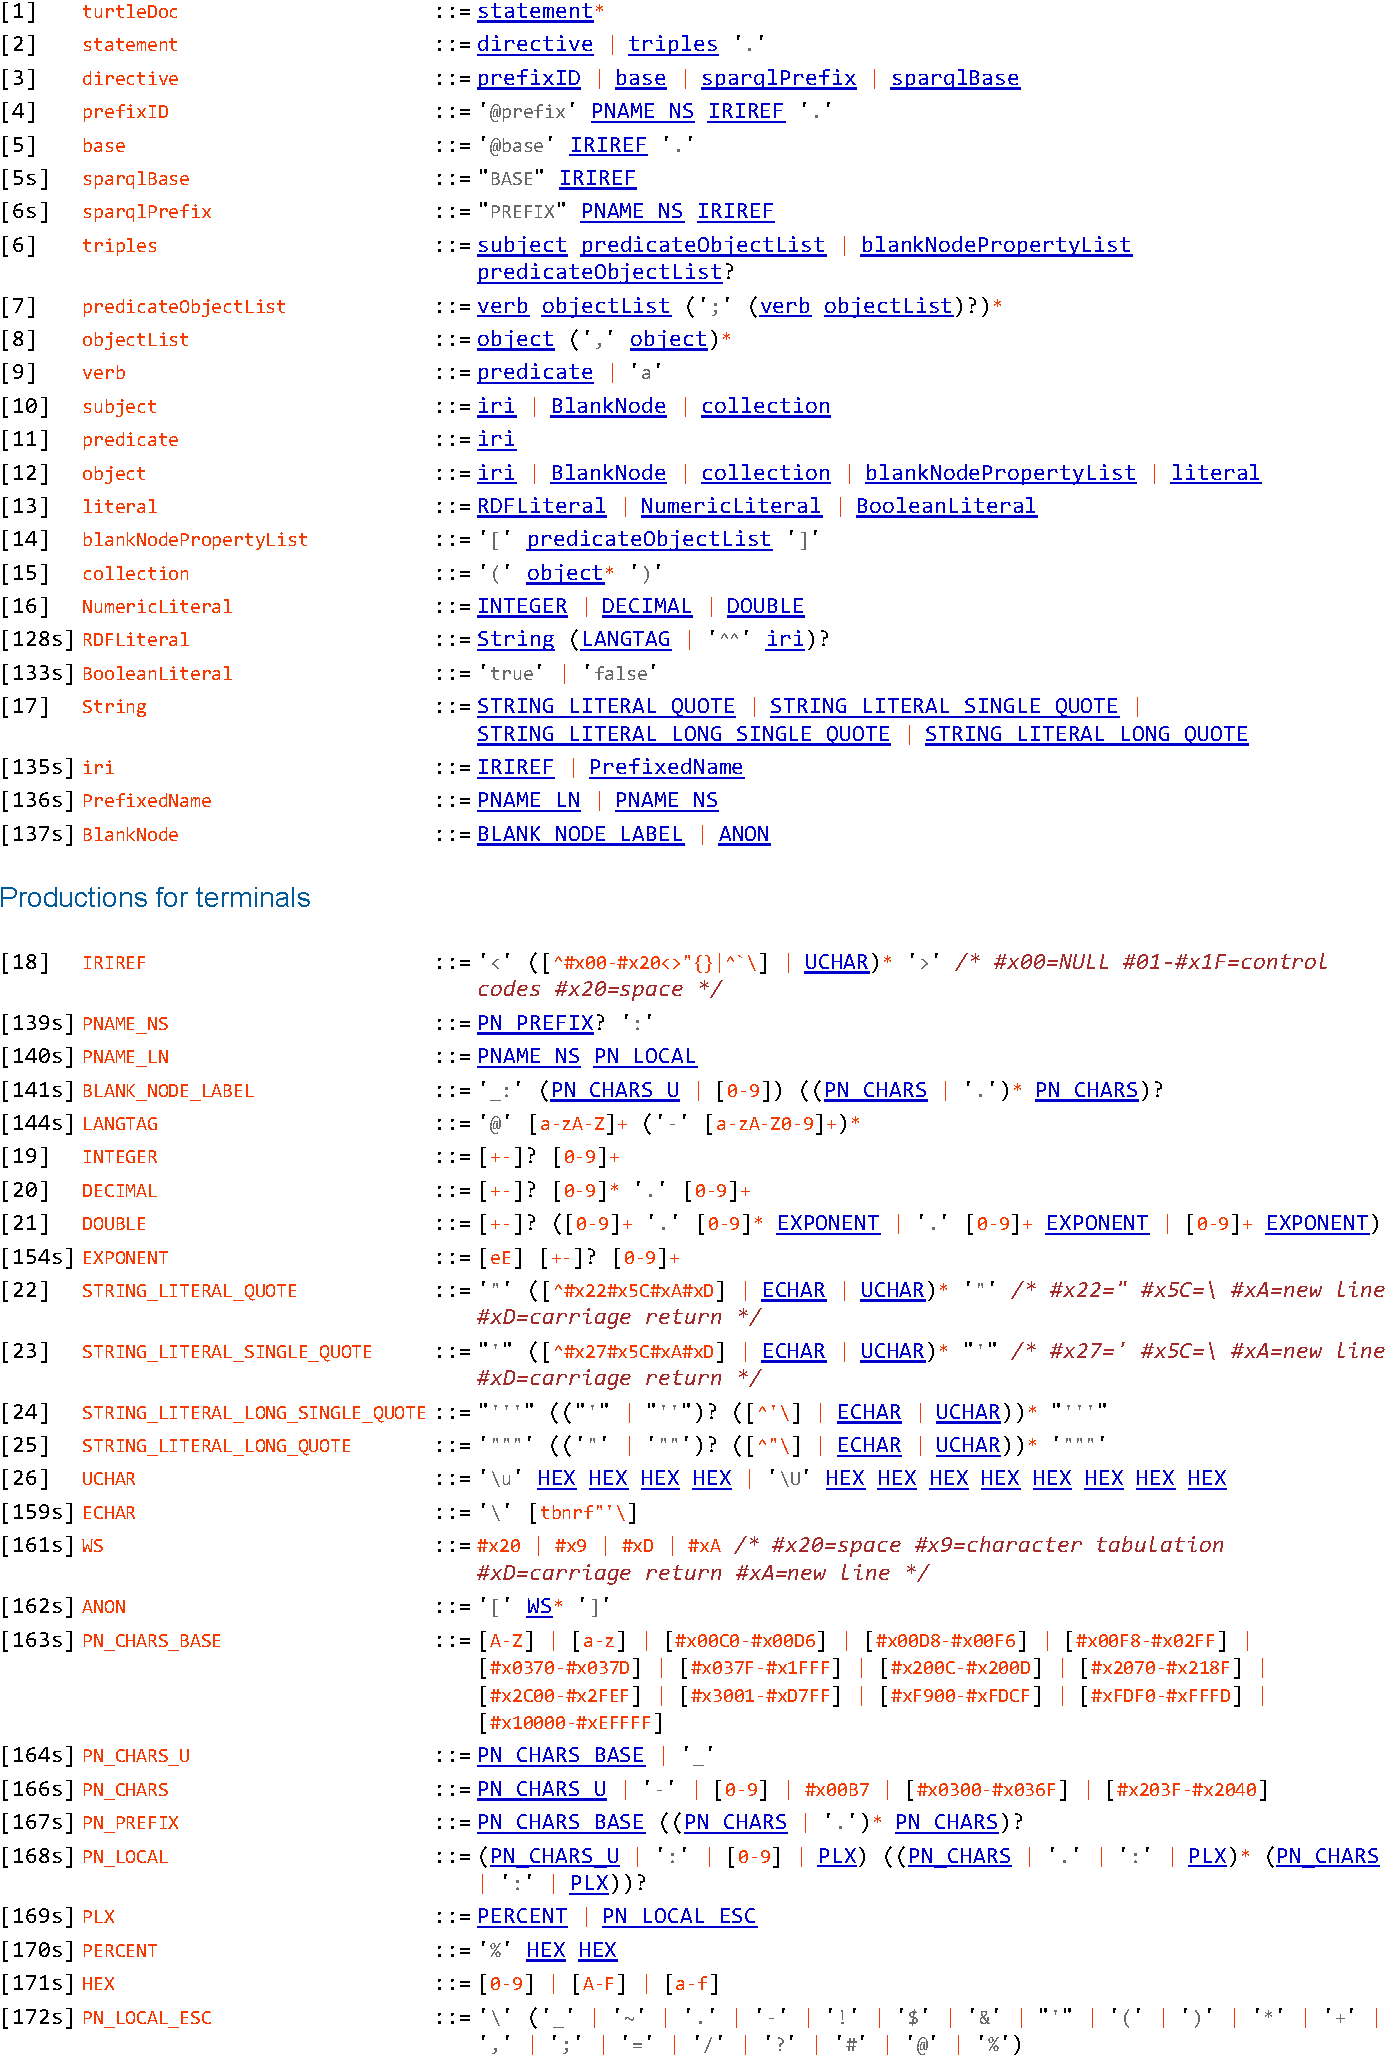
\includegraphics[width=\linewidth,height=\textheight,keepaspectratio]{Turtle_Grammar.pdf}

Notes:
\begin{itemize}
	\item [] Keywords in single quotes ('\texttt{@base}', '\texttt{@prefix}', '\texttt{a}', '\texttt{true}', '\texttt{false}') are case-sensitive. Keywords in double quotes ("\texttt{BASE}", "\texttt{PREFIX}") are case-insensitive. 
	\item [] Escape sequences \texttt{UCHAR} and \texttt{ECHAR} are case sensitive. 
	\item [] When tokenizing the input and choosing grammar rules, the longest match is chosen. 
	\item [] The Turtle grammar is LL(1) and LALR(1) when the rules with uppercased names are used as terminals. 
	\item [] The entry point into the grammar is \texttt{turtleDoc}. 
	\item [] In signed numbers, no white space is allowed between the sign and the number. 
	\item [] The strings '\texttt{@prefix}' and '\texttt{@base}' match the pattern for \texttt{LANGTAG}, though neither "\texttt{prefix}" nor "\texttt{base}" are \href{http://www.iana.org/assignments/language-subtag-registry}{registered language subtags}. This specification does not define whether a quoted literal followed by either of these tokens (e.g. \texttt{"A"@base}) is in the Turtle language. 
\end{itemize}

These rules describe the whole Turtle grammar.\\
Although we needed only the A-Box part, we decided to implement the whole grammar and to trigger only the rules needed for the A-Box part.

Therefore, we used only the rules: \texttt{1}, \texttt{4}, \texttt{5}, \texttt{9}, \texttt{10}, \texttt{11}, \texttt{12}, \texttt{13}, \texttt{16}, \texttt{128s}, \texttt{133s}, \texttt{135s}, and almost all the productions for terminals.

We translated these rules into the languages of Flex and Bison.\\
The translation was not straightforward for several reasons:
\begin{itemize}
	\item Flex does not support whitespaces among the tokens
	\item Flex does not support Unicode and as problems with Unicode ranges and they are essential in the Turtle format
	\item Flex does not support single quotes for the strings in the tokens
	\item Flex does not support different cases for different rules/tokens
	\item In Flex some characters, even if encoded in strings, needs to be escaped
	\item Flex has problems with “multi-levels” definitions
	\item In Flex the order of rules is important and affects the lexical analysis procedure
	\item Bison does not support single quotes for strings longer than one character (as in the C syntax)
	\item Bison has problems with strings (encoded in quotes) in the rules
	\item Bison does not support the Kleene star (\texttt{*}) and Kleene plus (\texttt{+})
	\item Bison does not support the optional operator (i.e. the question mark \texttt{?})
\end{itemize}

We employed the parsing procedure described in the Specification\footnote{\url{https://www.w3.org/TR/turtle/\#sec-parsing}}.

The RDF 1.1 Concepts and Abstract Syntax specification defines three types of RDF Term, but we consider only the first 2: IRIs, literals. Literals are composed of a lexical form and an optional language tag or datatype IRI. An extra type, prefix, is used during parsing to map string identifiers to namespace IRIs. Grammar productions change the parser state and emit triples.

Parsing Turtle requires a state of five items:
\begin{itemize}
	\item \texttt{IRI baseURI} — When the base production is reached, the second rule argument, \texttt{IRIREF}, is the base URI used for relative IRI resolution. 
	\item \texttt{Map[prefix -> IRI] namespaces} — The second and third rule arguments (\texttt{PNAME\_NS} and \texttt{IRIREF}) in the prefixID production assign a namespace name (\texttt{IRIREF}) for the prefix (\texttt{PNAME\_NS}). Outside of a \texttt{prefixID} production, any \texttt{PNAME\_NS} is substituted with the namespace. Note that the prefix may be an empty string, per the \texttt{PNAME\_NS} production: \texttt{(PN\_PREFIX)? ":"}. 
	\item \texttt{RDF\_Term curSubject} — The \texttt{curSubject} is bound to the subject production.
	\item \texttt{RDF\_Term curPredicate} — The \texttt{curPredicate} is bound to the verb production.\\
	If token matched was "\texttt{a}", \texttt{curPredicate} is bound to the IRI\\
	\texttt{http://www.w3.org/1999/02/22-rdf-syntax-ns\#type}.
\end{itemize}

Productions and lexical tokens to RDF terms or components of RDF terms are mapped as reported in \href{https://www.w3.org/TR/turtle/#sec-parsing-terms}{this section}.

A Turtle document defines an \href{http://www.w3.org/TR/rdf11-concepts/#dfn-rdf-graph}{RDF graph} composed of set of \href{http://www.w3.org/TR/rdf11-concepts/#dfn-rdf-triple}{RDF triple}s. The \href{https://www.w3.org/TR/turtle/#grammar-production-subject}{subject} production sets the \texttt{curSubject}.
The \href{https://www.w3.org/TR/turtle/#grammar-production-verb}{verb} production sets the \texttt{curPredicate}.
Each \href{https://www.w3.org/TR/turtle/#grammar-production-object}{object} \texttt{N} in the document produces an RDF triple: \texttt{curSubject curPredicate N}.

The approach to translate ABox RDF triples into ASP facts is described in \ste{Fix section reference}

\subsection{Integration of the parser in I-DLV}


\section{Activity title}
TODO
\chapter{Results}
\chapter{Open research issues}
\chapter{Bibliography}
\chapter{Appendix}


%%%%%%%%%%%%%%%%%%%%%%%%%%%%%%%%%%%%%%%%%%%%%%%%%%%%%%%%%%%%%%%%%%%%%%%%%%%%%%%%%%%%%%%%%%%%%%%%%%%%%%%%%%%%%%%%%%%%%%%%
%%%%%%%%%%%%%%%%%%%%%%%%%%%%%%%%%%%%%%%%%%%%%%%%%%%%%%%%%%%%%%%%%%%%%%%%%%%%%%%%%%%%%%%%%%%%%%%%%%%%%%%%%%%%%%%%%%%%%%%%
%%%%%%%%%%%%%%%%%%%%%%%%%%%%%%%%%%%%%%%%%%%%%%%%%%%%%%%%%%%%%%%%%%%%%%%%%%%%%%%%%%%%%%%%%%%%%%%%%%%%%%%%%%%%%%%%%%%%%%%%

\setcounter{chapter}{0}

\part*{Work Package 2:\\Enhancing the Query Rewriting Techniques}
\addcontentsline{toc}{part}{WP2: Enhancing the Query Rewriting Techniques}

\chapter{Scenario and problem description}

We aim at extending DLV for answering Conjunctive Queries (CQs) over Horn-SHIQ ontologies by following a Datalog-rewriting approach. To this aim, nice algorithms have been introduced in the literature in the last few years. One of the goals of WP2 is to design and develop an optimized algorithm for (Datalog-)rewriting CQs over Horn-SHIQ ontologies, after studying state-of-the-art approaches proposed in the literature. Moreover, WP2 aims at improving the existing DLV rewriting technique called Magic Sets for dealing with Datalog-rewritings of OWL knowledge bases. 
BLA BLA BLA…

\section{Team}
WP2 has been jointly performed by DLVSystem, SRUK and DeMaCS@UNICAL. In particular, what follows is the list of the involved researchers: Mario Alviano (Professor), Cristina Civili (PostDoc), Marco Manna (Professor), Pierfrancesco Veltri (PostDoc).

\section{Activity title}
TODO
\section{Activity title}
TODO
\section{Design Magic Sets enhanced for Datalog-rewriting of OWL ontologies. (Datalog to Datalog) - Activity 2.3}
Magic Sets are an optimization technique for addressing query answering in relational databases and logic-based systems. The technique is translational, from Datalog to Datalog in the context of this project, and therefore implementable as a module (almost) independent from other modules of DLV. The logic program in input is rewritten so that the subsequent bottom-up evaluation only materializes ground atoms that are relevant to answer the query in input. To this aim, new predicates are introduced in the rewritten program. Below is an example involving a recursive definition and asking for the descendants of mario:
\begin{verbatim}
  ancestor(X,Y) :- parent(X,Y).
  ancestor(X,Y) :- parent(X,Z), ancestor(Z,Y).
  ancestor(mario,X)?
\end{verbatim}

The Magic Sets rewriting starts with the query seed {\tt m\#ancestor\#bf(mario)}, modifies the rules defining the intentional predicate ancestor, and introduces magic rules for every occurrence of intentional predicates in the modified rules. The rewritten program is the following:
\begin{verbatim}
  m#ancestor#bf(mario).
  ancestor(X,Y) :- m#ancestor#bf(X), parent(X,Y).
  ancestor(X,Y) :- m#ancestor#bf(X),parent(X,Z),ancestor(Z,Y).
  m#ancestor#bf(Z) :- m#ancestor#bf(X), parent(X,Z).
\end{verbatim}

The rewritten program above is optimized for answering the specific query as its bottom-up evaluation only materializes descendants of mario, rather than the full ancestor relation.

There are cases in which several predicates for each predicate in the original program are introduced in the rewritten program. Below is an example, where all predicates are intentional, bindings are passed from left to right, and only rules defining the query predicate q are shown.
\begin{verbatim}
  q(X) :- r(a,X), s(X,Y), q(Y).
\end{verbatim}

The Magic Sets rewriting starts by introducing the magic seed {\tt m\#q\#f}. For each new predicate introduced by the rewriting, modified versions of the rules in input are added:
\begin{verbatim}
  q(X) :- m#q#f, r(a,X), s(X,Y), q(X).
\end{verbatim}
For each occurrence of an intentional predicate in a modified rule, a magic rule is added, possibly generating new predicates:
\begin{verbatim}
  m#r#bf(a) :- m#q#f.
  m#s#bf(X) :- m#q#f, r(a,X).
  m#q#b(Y) :- m#q#f, r(a,X), s(X,Y).
\end{verbatim}
The process is repeated, and the following rules are added:
\begin{verbatim}
  q(X) :- m#q#b(X), r(a,X), s(X,Y), q(X).
  m#r#bb(a,X) :- m#q#b(X).
  m#s#bf(X) :- m#q#b(X), r(a,X).
  m#q#b(Y) :- m#q#b(X), r(a,X), s(X,Y).
\end{verbatim}
At this point the rewriting reaches a fixpoint and terminates. Hence, the rewritten program contains the following rules (recall that the example is focused on the rules defining q, while the rules defining other intentional predicates have been omitted):
\begin{verbatim}
  m#q#f.
  q(X) :- m#q#f, r(a,X), s(X,Y), q(X).
  m#r#bf(a) :- m#q#f.
  m#s#bf(X) :- m#q#f, r(a,X).
  m#q#b(Y) :- m#q#f, r(a,X), s(X,Y).
  q(X) :- m#q#b(X), r(a,X), s(X,Y), q(X).
  m#r#bb(a,X) :- m#q#b(X).
  m#s#bf(X) :- m#q#b(X), r(a,X).
  m#q#b(Y) :- m#q#b(X), r(a,X), s(X,Y).
\end{verbatim}
Note that similar rules are introduced for predicates originating from the same source. Hence, a drawback of Magic Sets is the possible introduction of redundant rules and predicates.

Another possible source of inefficiency is the presence or the introduction of subsumed rules, that is, rules whose ground instances are included or less general than those associated with another rule in the program. Below is an example.
\begin{verbatim}
  q(X) :- p(X).
  q(X) :- p(X), t(X).
  q(a) :- p(a).
\end{verbatim}
We can observe that the first rules subsumes the other rules: ground instances of the second rule are less general than those of the first rule; the only ground instance of the third rule is among the the ground instances of the first rule.

\chapter{Results}
[...]

Concerning Activity 2.3, our goal is to further optimize the Magic Sets technique by introducing postprocessing modules that identify redundant rules and predicates. Specifically, redundant rules are identified by a module that checks for subsumption, that is, rules whose ground instances are included or less general than those associated with another rule in the program are removed; the number of pairs of rules to be checked is significantly reduced by means of hashing techniques. Below is the result of the application of such a module to the example given in Section 2.3. 
\[
\begin{array}{l}
{\tt q(X) :- p(X).}\\
\mathtt{\stkout{q(X) :- p(X), t(X).}}\\
\mathtt{\stkout{ q(a) :- p(a).}}\\
\end{array}
\]


Intuitively, given two rules $r_1$, $r_2$, subsumption $r_1 \sqsubseteq r_2$ is checked by means of a backtracking procedure that searches for a substitution of the variables of r1 such that the head of $r_1$ matches the head of $r_2$, and the body of $r_1$ is a subset of the body of $r_2$. If such a substitution is found, rule  $r_2$ is removed. Checking all pairs is too expensive, and therefore each rule is associated with an hash value, currently of size 64 bits, computed as follows:
\begin{itemize}
\item <OR of IDs of head predicates>, 8 bits;
\item <OR of IDs of head constants>, 8 bits;
\item <OR of IDs of predicates in positive body>, 16 bits;
\item <OR of IDs of constants in positive body>, 16 bits;
\item <OR of IDs of predicates in negative body>, 8 bits;
\item <OR of IDs of constants in negative body>, 8 bits.
\end{itemize}
Subsumption $r_1 \sqsubseteq r_2$ is checked only if the following bit-a-bit equation is satisfied:
$$hash(r_1) \ \& \ hash(r_2) == hash(r_1)$$
In the example above, the third rule cannot subsume the other rules because of the constant a, and the second rule cannot subsume the other rules because of the predicate t; depending on the IDs associated with predicates and constants, the hashing technique can detect this fact and avoid the backtracking searches.

The module that identifies redundant predicates, instead, takes into account the different bindings associated with predicates originating from the same source, and eliminates the rules associated with the more bounded predicates. In the example given in Section 2.3, predicate {\tt m\#q\#b} is more bounded than predicate {\tt m\#q\#f}, and therefore the rules associated with {\tt m\#q\#b} are removed. Similarly, rules associated with {\tt m\#r\#bb} and {\tt m\#s\#bf} are removed. Hence, the rewritten program, focused on the rules defining q, is the following:
\[
\begin{array}{l}
	{\tt m\#q\#f.}\\
	{\tt q(X) :- m\#q\#f, r(a,X), s(X,Y), q(X).}\\
	{\tt m\#r\#bf(a) :- m\#q\#f.}\\
	{\tt m\#s\#bf(X) :- m\#q\#f, r(a,X).}\\
	\mathtt{\stkout{m\#q\#b(Y) :- m\#q\#f, r(a,X), s(X,Y).}}\\
	\mathtt{\stkout{q(X) :- m\#q\#b(X), r(a,X), s(X,Y), q(X).}}\\
	\mathtt{\stkout{m\#r\#bb(a,X) :- m\#q\#b(X).}}\\
	\mathtt{\stkout{m\#s\#bf(X) :- m\#q\#b(X), r(a,X).}}\\
	\mathtt{\stkout{m\#q\#b(Y) :- m\#q\#b(X), r(a,X), s(X,Y).}}\\
\end{array}
\]
[...]



\chapter{Open research issues}
\chapter{Bibliography}
\chapter{Appendix}


%%%%%%%%%%%%%%%%%%%%%%%%%%%%%%%%%%%%%%%%%%%%%%%%%%%%%%%%%%%%%%%%%%%%%%%%%%%%%%%%%%%%%%%%%%%%%%%%%%%%%%%%%%%%%%%%%%%%%%%%
%%%%%%%%%%%%%%%%%%%%%%%%%%%%%%%%%%%%%%%%%%%%%%%%%%%%%%%%%%%%%%%%%%%%%%%%%%%%%%%%%%%%%%%%%%%%%%%%%%%%%%%%%%%%%%%%%%%%%%%%
%%%%%%%%%%%%%%%%%%%%%%%%%%%%%%%%%%%%%%%%%%%%%%%%%%%%%%%%%%%%%%%%%%%%%%%%%%%%%%%%%%%%%%%%%%%%%%%%%%%%%%%%%%%%%%%%%%%%%%%%
\setcounter{chapter}{0}

\part*{Work Package 3:\\Enhancing the SPARQL Query Evaluation/Execution Procedure}
\addcontentsline{toc}{part}{WP3: Enhancing the SPARQL Query Evaluation/Execution}

\chapter{Scenario and problem description}

DLV has been designed as an in-memory system allowing only one-shot executions. In particular, when it is run on a specific input the system starts, loads input data, processes the requested query and stops as soon as the computation is completed. However, when multiple queries are evaluated over the same input data, the aforementioned behaviour could be rather expensive since the system needs to reload input data at each run and for each query. Within WP3, we aim at extending the system by providing a server-like behaviour that allows to keep the main process alive also after the computation is performed. In this way, DLV will be able to answer multiple queries over the same input knowledge base without loading input data more than once. More in detail, we plan to further equip the DLV server version with the following useful functionalities:
\begin{itemize}
\item Load ontology
\item Load data (in form of logic fact or RDF triple)
\item Add data (in form of logic fact or RDF triple)
\item Remove data (in form of logic fact or RDF triple)
\item Run query
\item Reset ontology
\item Reset data
\item Compute statistics for query optimizations
\end{itemize}

A further goal of WP3 is to study and develop suitable optimization techniques intended to speed-up the execution of query-programs on given query-patterns (e.g., advanced indexing and ordering techniques). Finally, the last goal of this work package is to reduce the memory consumption of DLV in order to permit the handling of large scale knowledge bases characterized by ABoxes featuring billions of triples.
BLA BLA BLA… 



\section{Team}
WP3 has been jointly developed by DLVSystem and DeMaCS@UNICAL. In particular, what follows is the list of the involved researchers: Francesco Calimeri (Professor), Roberta Costabile (PhDStudent), Alessio Fiorentino (PhDStudent), Davide Fuscà (PostDoc), Simona Perri (Professor), Kristian Reale (PostDoc), Francesco Ricca (Professor), Jessica Zangari (PostDoc).

\section{Activity title}
TODO
\section{Activity title}
TODO
\section{Activity title}


\chapter{Results}
\chapter{Open research issues}
\chapter{Bibliography}
\chapter{Appendix}

%%%%%%%%%%%%%%%%%%%%%%%%%%%%%%%%%%%%%%%%%%%%%%%%%%%%%%%%%%%%%%%%%%%%%%%%%%%%%%%%%%%%%%%%%%%%%%%%%%%%%%%%%%%%%%%%%%%%%%%%
%%%%%%%%%%%%%%%%%%%%%%%%%%%%%%%%%%%%%%%%%%%%%%%%%%%%%%%%%%%%%%%%%%%%%%%%%%%%%%%%%%%%%%%%%%%%%%%%%%%%%%%%%%%%%%%%%%%%%%%%
%%%%%%%%%%%%%%%%%%%%%%%%%%%%%%%%%%%%%%%%%%%%%%%%%%%%%%%%%%%%%%%%%%%%%%%%%%%%%%%%%%%%%%%%%%%%%%%%%%%%%%%%%%%%%%%%%%%%%%%%
\setcounter{chapter}{0}

\part*{Work Package 4:\\Test Case Design}
\addcontentsline{toc}{part}{WP4: Test Case Design}

\chapter{Scenario and problem description}

Within activity A4.1, we aim at building a benchmark domain for evaluating powerful ontology reasoners relying on a non-materialization approach over a large dataset (more than 1 billion triples), where the latter is constantly subject to evolution (addition or deletion of triples from the ABox). The goal of this activity is to appropriately select and extend, if possible, an existing OWL benchmark for evaluating ontology reasoners against a large knowledge base with (near-)real time data. In particular, we must consider only benchmarks that enjoy the following main requirements:
\begin{enumerate}
\item the data generator is able to generate more than 1 billion triples;
\item the ontology expressiveness is as close as possible to OWL 2 DL;
\item the benchmark evaluates the tested systems over a dynamic dataset. 
\end{enumerate}
In order to simulate a dynamic evolution of the knowledge base, the tested systems will be required to load an initial large dataset (close to 1 billion triples) and answer a fixed set of queries. Next, at a frequency $f=\frac{1}{\Delta T}$ where $\Delta T$ is a given time period,  $x\%$ of the initial number of triples will be either deleted or generated and added to the ABox. After the systems are notified of the underlying knowledge base changes, they will have to answer again the fixed set of queries. Hence, the frequency $f$ and the rate $x\%$ (expressed as percentage of the initial number of triples) of the instance deletions/additions should be a tuneable parameter of our benchmark. 

Currently, the research effort provide a number of well-established benchmarks, including LUBM, UOBM, BSBM and SPB. LUBM has been designed for comparing performance, soundness and completeness of OWL reasoning engines, against a static knowledge base. UOBM extends LUBM by adding axioms that make use of all OWL Lite and OWL DL constructs. BSBM aims at comparing the performances of systems that expose SPARQL endpoints, and can simulate different real-world scenarios. Similarly, the Semantic Publishing Benchmark (SPB) can simulate a real-world scenario where a number of aggregation agents provide the heavy query workload, while at the same time a steady stream of editorial agents execute a number of update operations.

According to the requirements introduced above, none of the aforementioned benchmarks can be used without being extended for our purpose. Indeed, UOBM features an ontology going beyond Horn-SHIQ and it does not provide any official (dynamic) data generator. BSBM includes some queries requiring either aggregates or string functions and it does not provide any way to simulate data evolution. SPB does provide a reliable data generator and it can simulate a dynamic environment but its ontology is too easy to handle since its expressiveness falls into OWL 2 RL. Finally, LUBM does not simulate a dynamic environment. 

However, this latter benchmark seems to be the most suitable choice since it could be easily extended for our purpose. Indeed, it provides an expressive ontology (falling into Horn-SHIQ and going beyond OWL 2 RL), a reliable data generator (which can be exploited to generate huge instances and to produce axioms to be added during the ABox evolution) and a set of 14 SPARQL queries.


Hence, the main goal of activity A4.1 is to equip LUBM with a test driver that allows simulating a dynamic evolution of the initial dataset, by adding/deleting $x\%$  of the initial number of triples at a frequency $f=\frac{1}{\Delta T}$ (notice that both $\Delta T$ and $x$ should be tuneable parameters of our test driver). Moreover, we aim at devising more complex queries to fully exploit expressiveness of the LUBM ontology since 9 out of the original 14 queries can be now handled by any OWL 2 RL reasoner.
BLA BLA BLA… 


\section{Team}
WP1 has been jointly developed by DLVSystem and SRUK. In particular, what follows is the list of the involved researchers: Pierfrancesco Veltri (PostDoc), Maud Lemercier (Software Engineer).

\section{Activity title (A4.1)}
TODO
\section{Activity title (A4.2)}
TODO
\section{Activity title (A4.3)}


\chapter{Results}
\chapter{Open research issues}
\chapter{Bibliography}
\chapter{Appendix}


\end{document}
